\documentclass{article}
\usepackage{tikz}
\usepackage{pgfplots}\pgfplotsset{compat=1.17}
\begin{document}
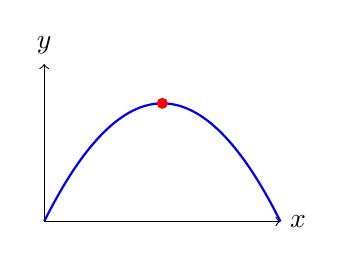
\begin{tikzpicture}
  \draw[->] (0,0) -- (3,0) node[right] {$x$}; \draw[->] (0,0) -- (0,2) node[above] {$y$};
  \draw[thick,blue] (0,0) .. controls (1,2) and (2,2) .. (3,0);
  \fill[red] (1.5,1.5) circle (2pt);
\end{tikzpicture}

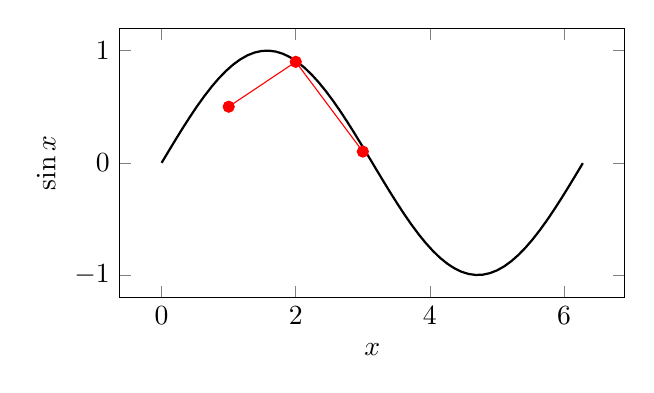
\begin{tikzpicture}
\begin{axis}[xlabel=$x$,ylabel=$\sin x$,width=8cm,height=5cm]
\addplot[domain=0:6.28,samples=60,thick]{sin(deg(x))};
\addplot[red,mark=*] coordinates {(1,0.5)(2,0.9)(3,0.1)};
\end{axis}
\end{tikzpicture}
\end{document}
